\chapter{Methodology}
\label{chp:Methodology} 

\section{Introduction}
This chapter serves as the foundation for the implementation phase for this study. It starts with introducing the requirements for the testbed, an introduction to the testbeds hardware and ends with an overview of its characteristics.

\section{Requirements}
The main objective for this project is to create a hybrid solution for testing \gls{its} application taking the advantages from the software simulation models, applying them on low-cost robots and taking the advantages from testing on real cars. In order for this to work we need to fulfill some requirements. Some systems like VANET and GPS needs to be emulated for indoor use. 

\subsection{List of requirements}
\begin{enumerate}
\item \textbf{Flexibility}: Support changes in simulation environment. Different map layouts. Multiple robots

\item \textbf{Communication}: Supplement of VANET/DSRC. Use WiFi. Find some requirements for latency.

\item \textbf{Dynamic Driving}: Cars take independent decisions. Decentralized decision making

\item \textbf{Real-world driving characteristics}: Route planing, speed adaption, awareness

\item \textbf{Localization}: Indoor GPS supplement

\item \textbf{Low Cost}: In order to be feasable 

\end{enumerate}

\section{DiddyBorg V2}
For this project the choice of robots is the DiddyBorg V2 robot which is an upgraded version from the DiddyBorg V1 previously used in Anders Brastad's thesis \cite{DevelopmentOfVTL}. DiddyBorg V2 is a 6 wheeled high-torque robotics platform powered with batteries. It uses six 12V DC gear motors with three mounted on each side of the robot. Its main controlling unit is an on board Raspberry Pi 3 making it highly customizable and suitable for this project. 

\noindent The DiddyBorg robots are one of the most powerful robots available on the market and is easily controlled through a Python API provided by the PiBorg Organization. It can drive over most indoor and outdoor terrain, is able to climb inclines up to 45 degrees and perform a 360 degree turn which makes it suitable for a testbed. Compared to existing solutions for testing \gls{its} application, the simulations can be executed indoor in a controlled environment as opposed to an outdoor test with more variability in its environment. The robots have a low cost - 210 pounds - and are easily customizable and extendable for new use-cases. Figure \ref{fig:diddyborg-robot} shows one of the assembled DiddyBorg robots. 

\begin{figure}[H]
\centering
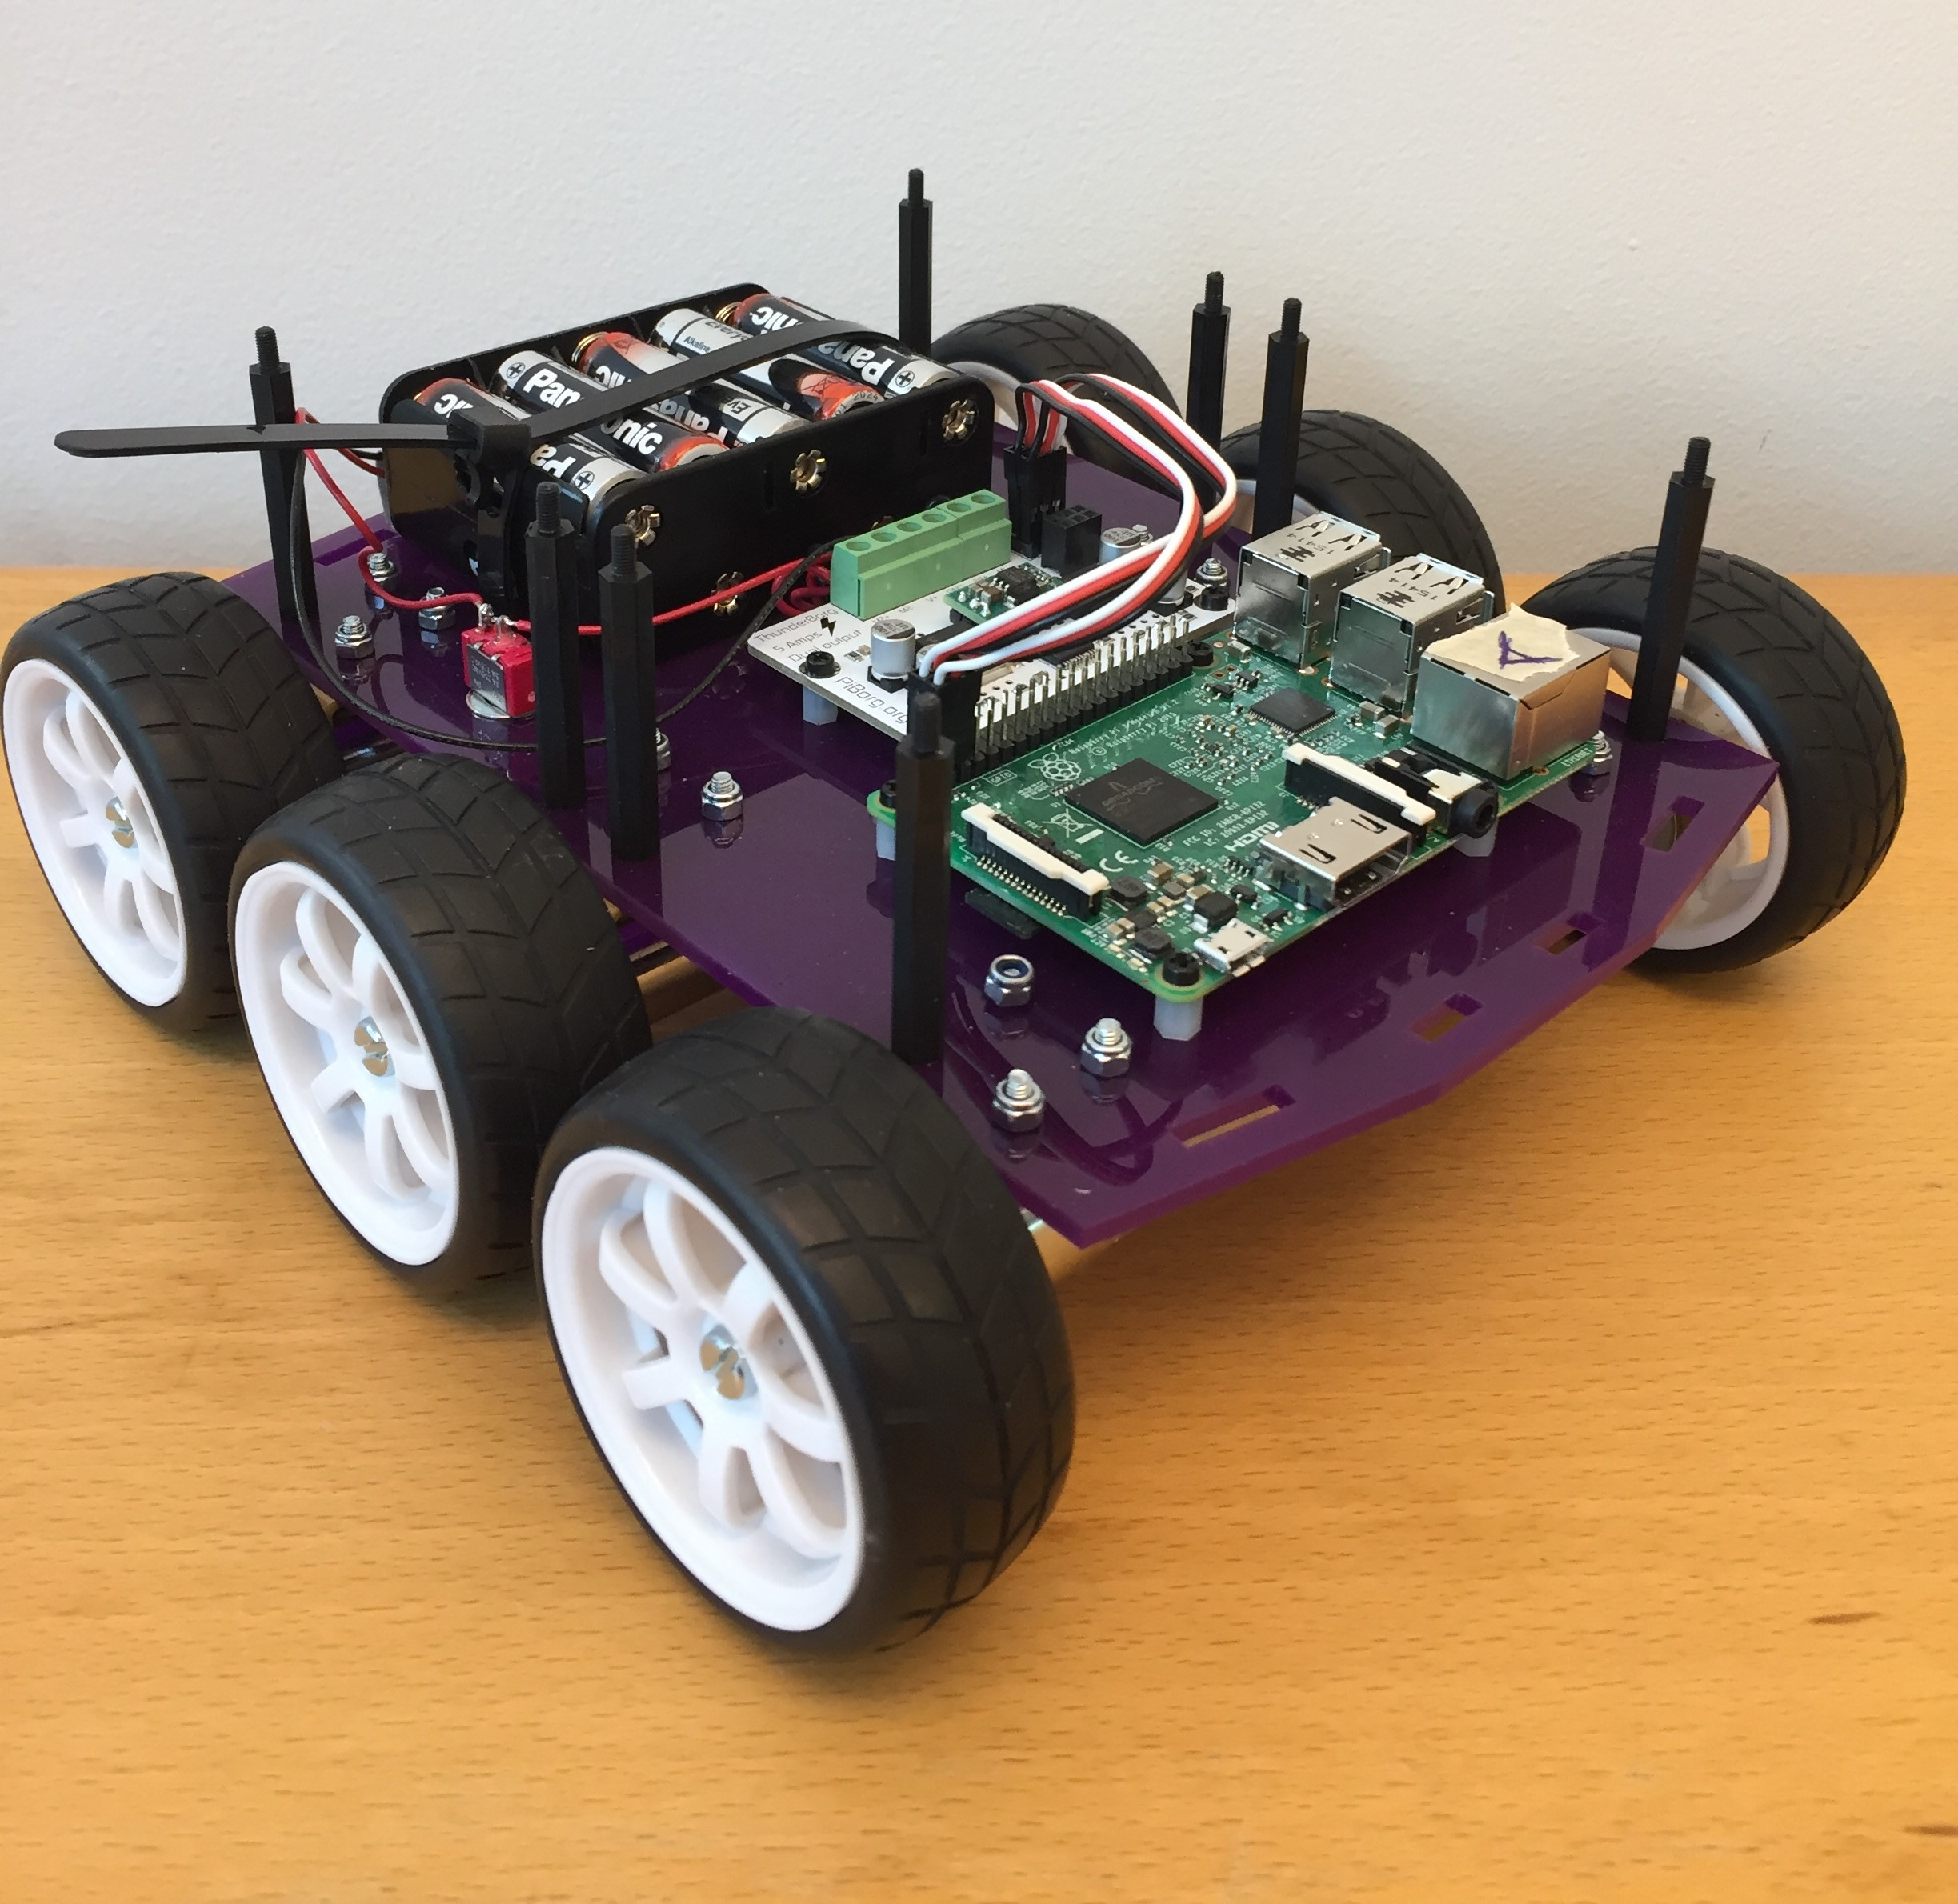
\includegraphics[width=10cm]{images/DiddyBorgV2.jpg}
\caption{Fully assembled DiddyBorg V2 robot}
\label{fig:diddyborg-robot}
\end{figure}

\subsection{Raspberry Pi 3}
Raspberry Pi 3 is a small credit-card-sized computer at a low cost. It can be used as a small personal computer, a media center or as a controlling unit in an electronics project. It comes with a variety of different Operating Systems which is chosen for different types of use. For this thesis the Raspberry Pi is installed with Raspbian as its Operating System. Raspbian is based on Debian and optimized for the Raspberry Pi hardware. It provides an easy to use GUI which makes development and configuration of the unit easier for this project. 

\textbf{Raspberry Pi 3 specifications}
\begin{itemize}
\item Quad Core 1.2GHz 64bit CPU
\item 1GB RAM
\item 4 USB 2 ports
\item Full size HDMI port
\item 40-pin extended GPIO
\item Wireless LAN and Bluetooth Low Energy on board
\item CSI camera port for Raspberry Pi Camera
\end{itemize}

\begin{figure}[H]
\centering
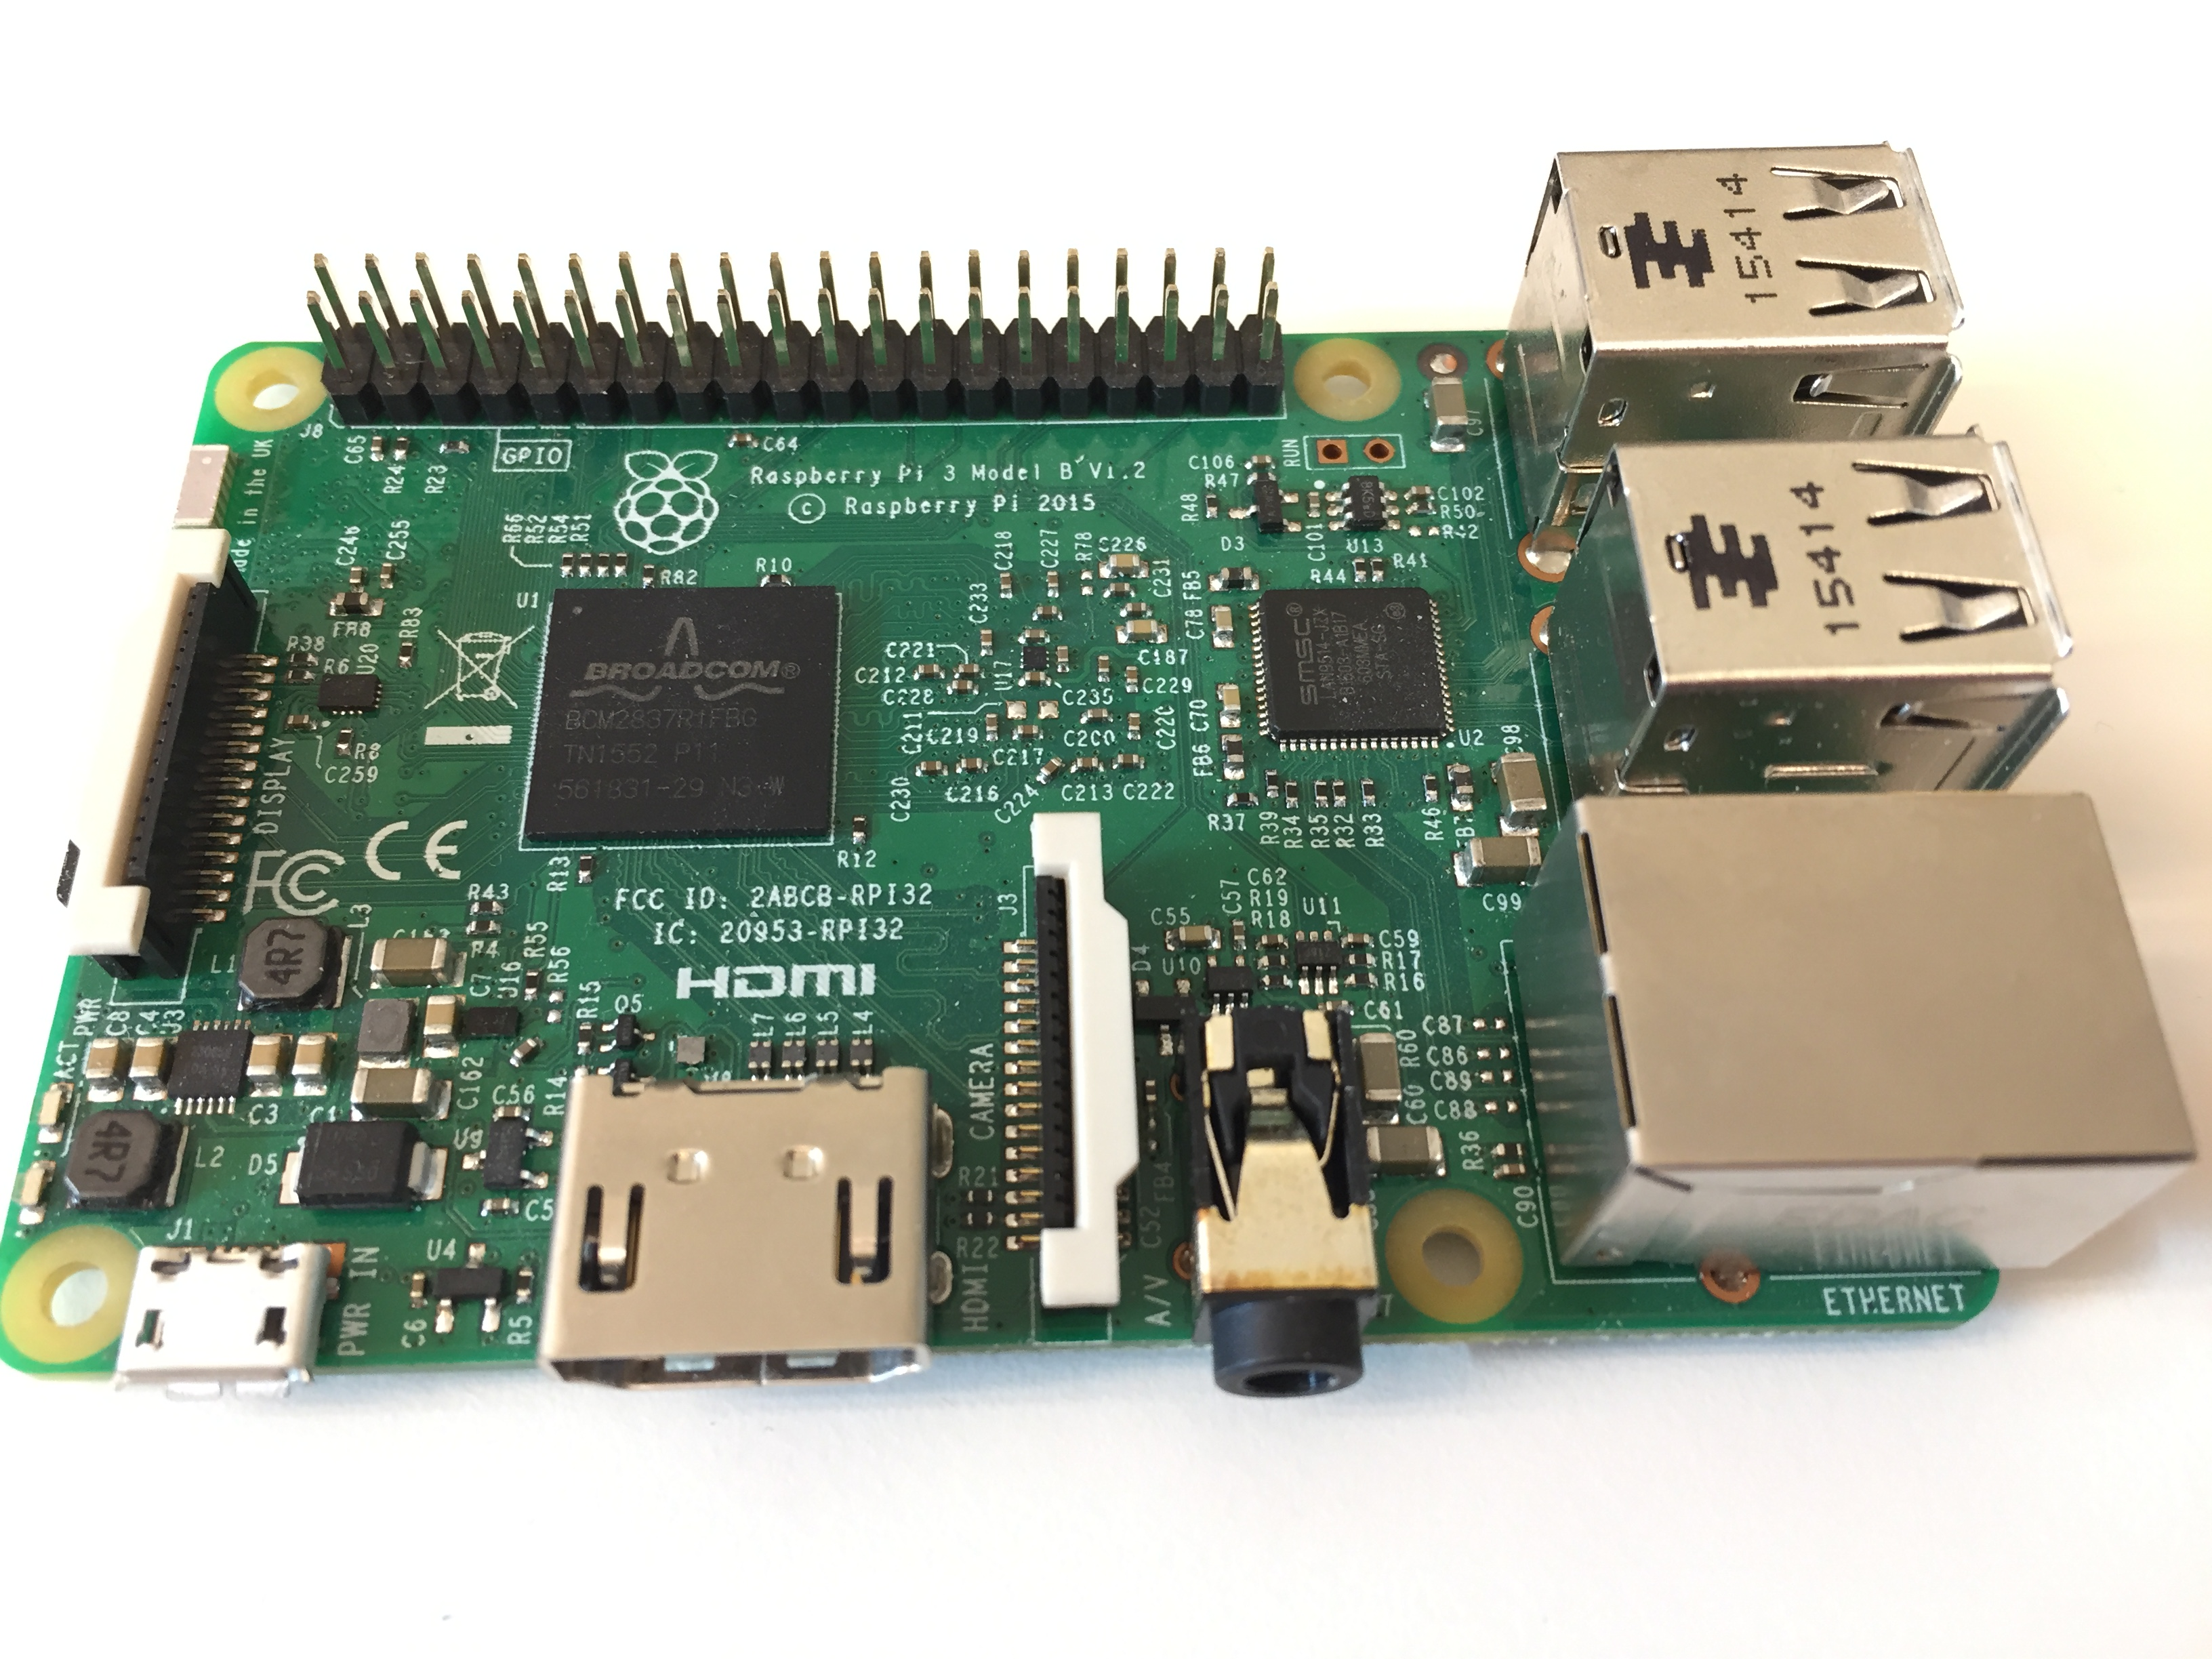
\includegraphics[width=10cm]{images/Raspi3.jpg}
\caption{Raspberry Pi 3}
\label{fig:raspberry-pi}
\end{figure}

\subsection{ThunderBorg}
ThunderBorg is a powerful dual motor control board which makes it possible to power the DiddyBorg motors and the Raspberry Pi with batteries instead of a USB supply. ThunderBorg is directly connected to all six motors and  to the Raspberry Pi via GPIO. The PiBorg organization also provides an easy to use Python API for controlling the motors. A list of available commands are listed in appendix \ref{appendix:thunderborg}. The ThunderBorg board is shown in figure \ref{fig:thunderborg}

\begin{figure}[H]
\centering
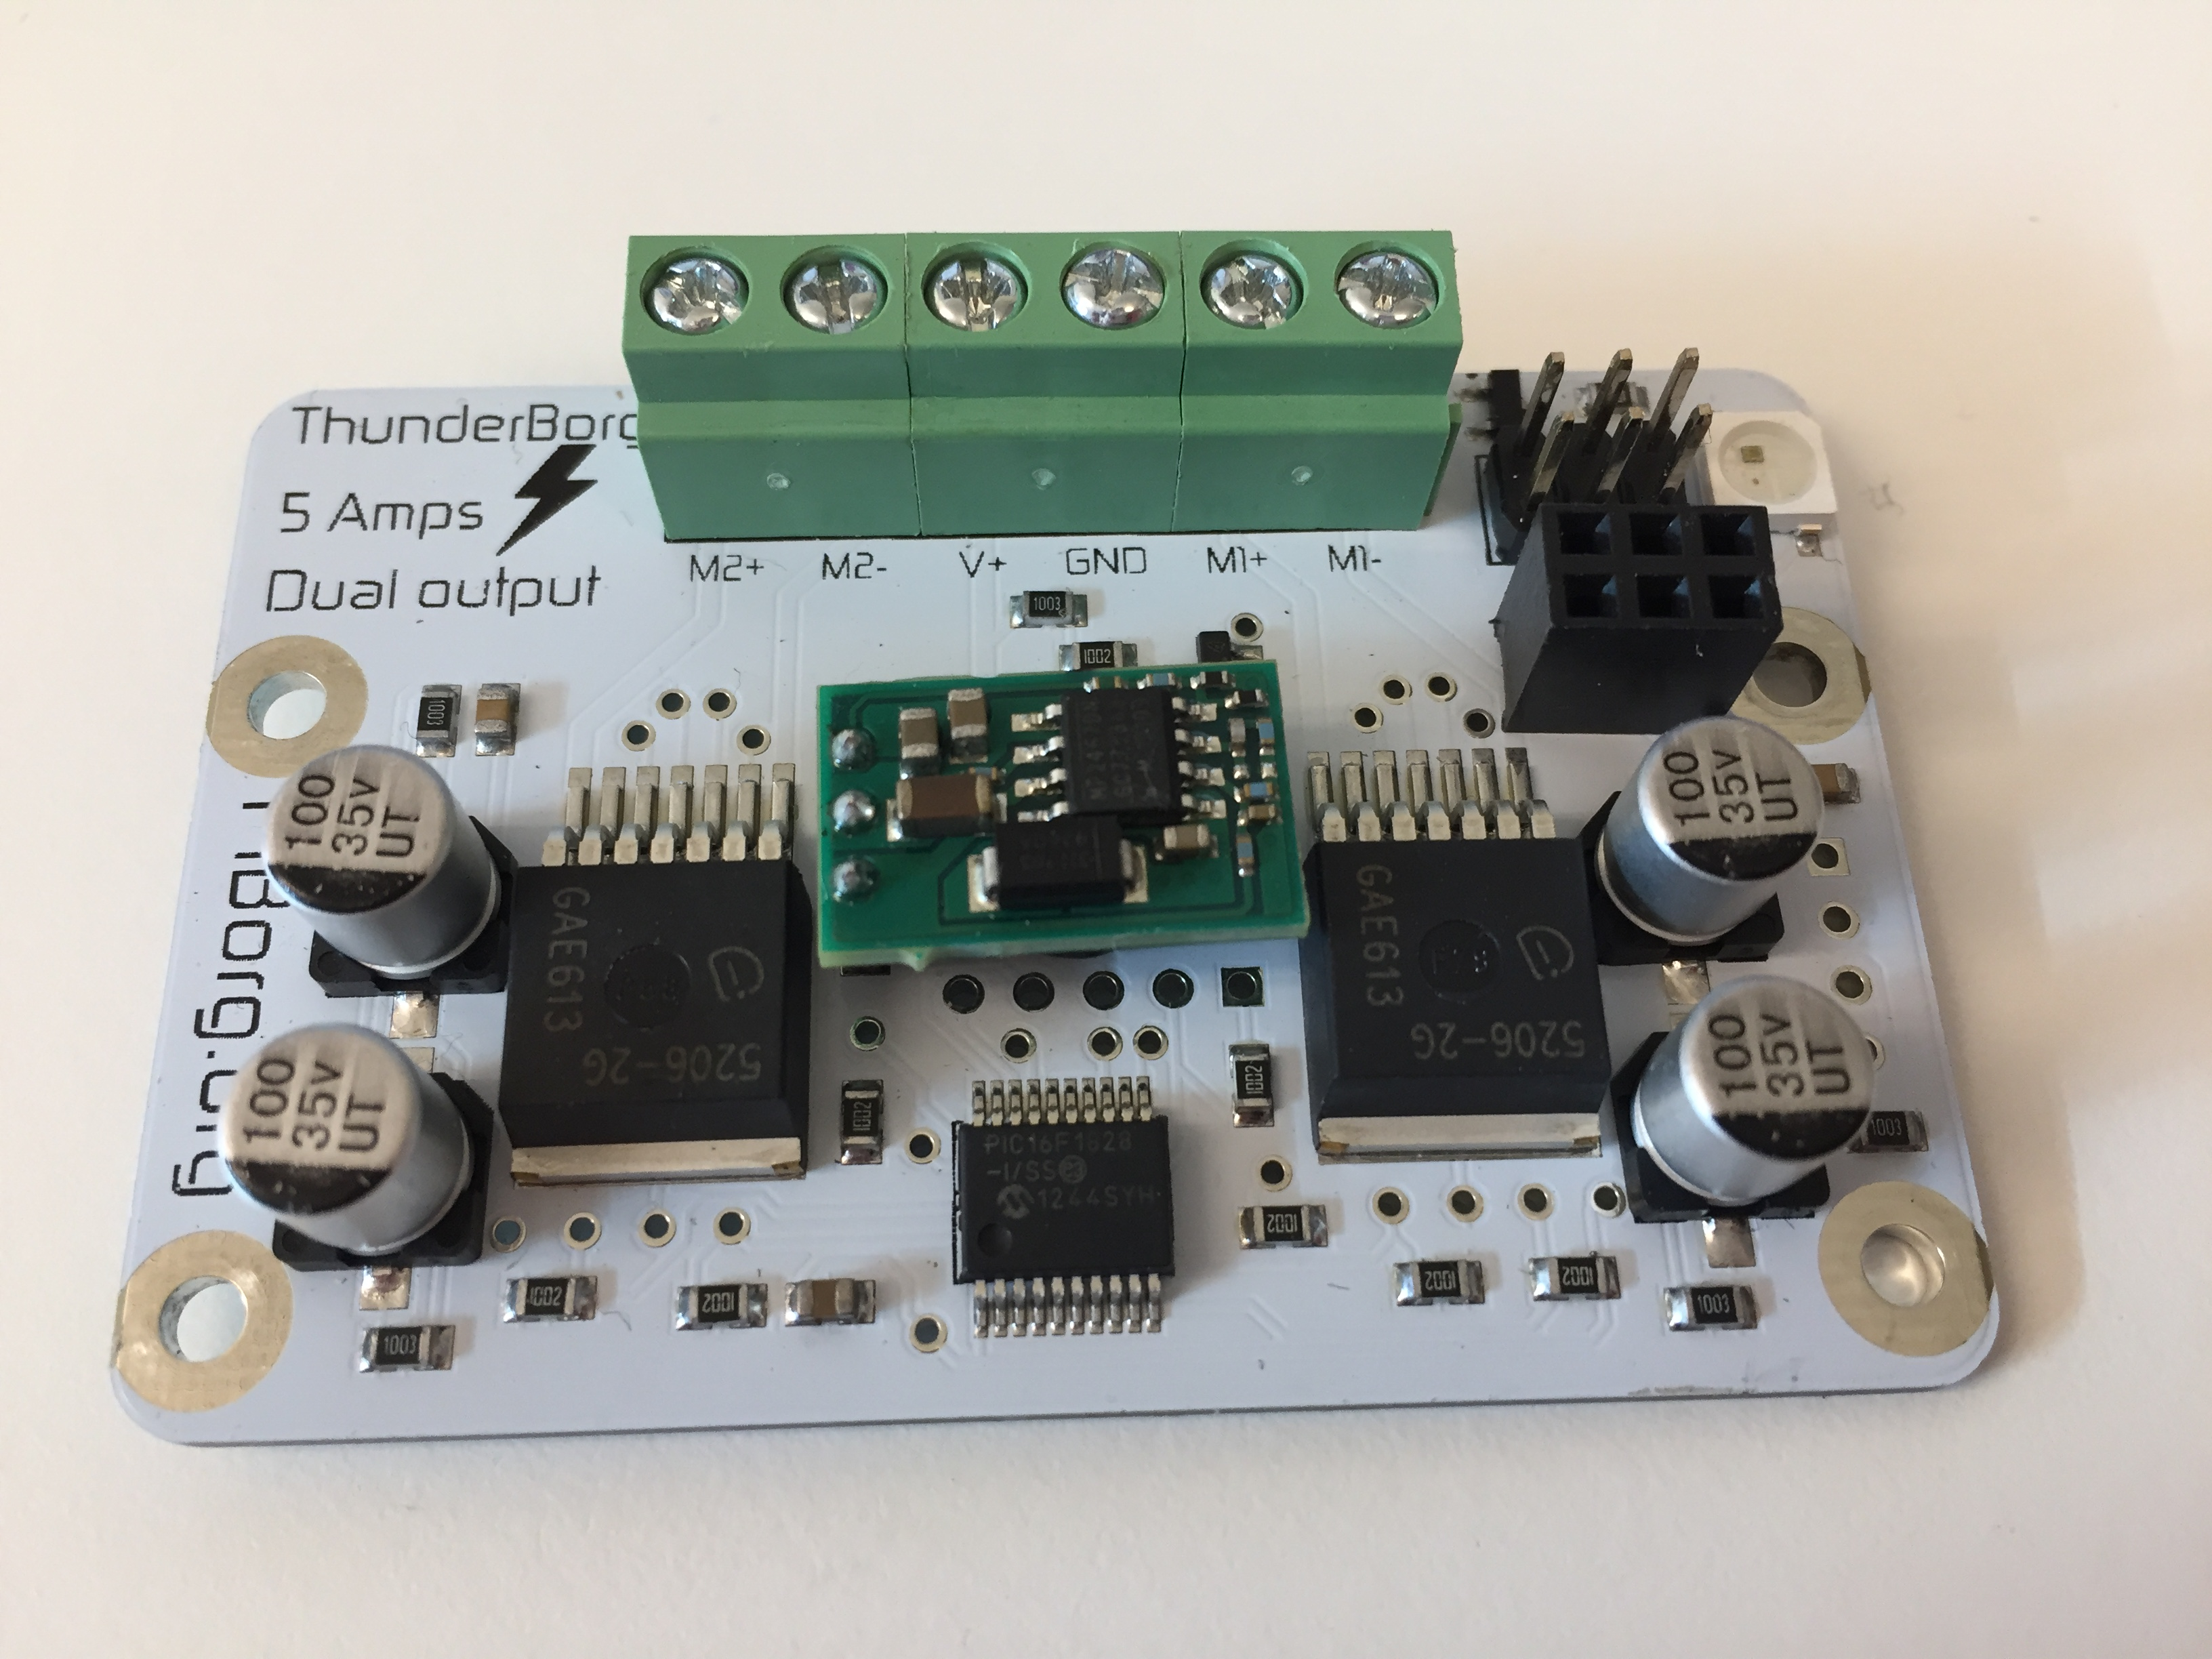
\includegraphics[width=10cm]{images/thunderborg.jpg}
\caption{ThunderBorg}
\label{fig:thunderborg}
\end{figure}

\subsection{Camera}
In order for the robots to have self-driving capabilities they are fitted with a Raspberry Pi Camera. This enables high-definition video for use with image recognition tools such as Lane Detection. The camera is mounted in front of the robot and is used as a solution for indoor localization/positioning. 

\section{Characteristics}
This sections describes some of the key characteristics for the testbed. These characteristics are needed in order to create a base platform to conduct tests and experiments. We need to implement much of the functionality that is and will be available on the market for \gls{its} to be realized in the future. For this project three main characteristics has been selected as the main objectives. 

\subsection{Semi-autonomous driving}
One key component for a traffic optimization testbed is that it needs to support changes in its simulation environment. All robots have an internal map of the surrounding
environment. By allowing this map to be replaced and changed for different simulation scenarios, mechanisms on the robot needs to be implemented. In the
current testbed implementation \cite{DevelopmentOfVTL}, the robots follow a fixed route, driving in a
loop. By allowing changes in environment these fixed routes needs to be dynamic.
\newline
\newline
Another important factor is that the system should simulate actual driving behavior
and support multiple robots. To achieve this multiple mechanisms must be implemented:
map exploration, handling out-of-bounds, indoor positioning, collaboration
between robots and simulation of actual driving behavior. Map exploration and out of bounds is described in section 4.3.

\subsection{Localization}
One key requirement for this projects is to have a system for indoor localization and positioning. For real-world scenarios Global Positioning System (GPS) is the preferred solution that fits the requirements for accuracy and latency. However, a GPS solution does not fit the requirements for this project as it has problems with indoor use and not accurate enough for this project. An indoor positioning system needs to be in place. Implementing a positioning system with software for computer simulations is considered easy and solved. A new problem arises as soon as the system have moving parts which introduces inaccuracy. If the system sends a command to the robot to turn 90 degrees without any confirmation, the robot might over or under turn by some degrees. This inaccuracy will potentially put the robot off course and out of bounds. The system needs to have some kind of component to correct the robots inaccuracy movements. After exploring multiple solutions such as digital compass, ready make indoor positioning system, the choice to use Lane Detection as a correction mechanism was taken. 

\subsubsection{Lane Detection}
Lane Detection is a mechanism used in self-driving cars to detect lanes on roads in real-time. For self-driving cars this method is used to keep the car in the middle of the lanes and to steer in bends. Interestingly, this method can be used as a tool to adjust the robots heading and increase the accuracy of the robots position with respect to the system. \cite{aziz_implementation_2017}

\noindent The process of Lane Detection is as follows:

\begin{enumerate}
    \item Take a frame captured by the Raspberry Pi Camera
    \item Apply an undistortion algorithm to remove camera distortion from the image
    \item Convert the image to gray scale to better separate lanes from roads
    \item Apply some Gaussian smoothing to remove noise on the image
    \item Use an edge detection algorithm (Canny Edge Detection) to detect edges in the image
    \item Trim the image to a region of interest
    \item Apply the Hough Transform algorithms to convert edges on image to physical points/lines in x, y pairs
    \item Apply some linear algebra to create two lines on the image, one for left lane and one for right lane
    \item Average the highest X value on the left lane and the lowest X value on the right lane to get a center point
    \item Compare the current center point to actual center point. If center is higher than actual center, turn slightly left and opposite if the center is lower than actual center
\end{enumerate}

\noindent Figure xx show the output image for each step in the algorithm.

\subsection{Simulate driving behaviour}
In order for the system to represent real-world scenarios it should mock some characteristics that represent normal driving behavior. For this project three key characteristics has been identified. 

\begin{enumerate}
\item \textbf{Route Planning}: Drivers usually drive a partially to fully planned route. This can be achieved by dynamically having a planned route for the robots which also enables a more seamless driving during simulations. 
\item \textbf{Speed Adaption}: When entering and exiting intersections drivers decelerate and accelerate their speed. 
\item \textbf{Consider other cars}: This is important to avoid accidents and to know where other robots are in order to take the correct action.
\end{enumerate}